\documentclass[crop,tikz,border=10px,convert=pdf2svg,multi=false]{standalone}
\usepackage[defaultsans]{opensans}
\usetikzlibrary{shapes,arrows,positioning}
\begin{document}
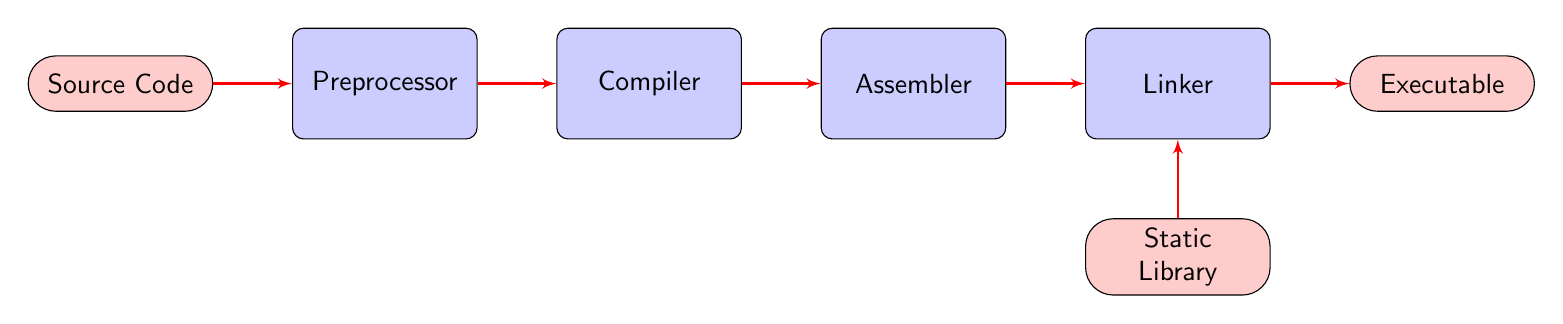
\begin{tikzpicture}[font=\sffamily,remember picture,
  block/.style = {rectangle, draw, fill=blue!20, text centered, text
    width=6em, rounded corners, minimum height=4em},
  cloud/.style = {rectangle, draw, fill=red!20, text centered, text
    width=6em, rounded corners=10pt, minimum height=2em},
  line/.style = {-latex', red, thick},
  title/.style = {draw=none, font=\Large\bf\sffamily, text centered}]

  \node [cloud] (src) {Source Code};
  \node [block, right=of src] (pp) {Preprocessor};
  \node [block, right=of pp] (compiler) {Compiler};
  \node [block, right=of compiler] (assembler) {Assembler};
  \node [block, right=of assembler] (linker) {Linker};
  \node [cloud, right=of linker] (exe) {Executable};

  \node [cloud, below=of linker] (static) {Static\\ Library};

  \draw [line] (src) -- (pp);
  \draw [line] (pp) -- (compiler);
  \draw [line] (compiler) -- (assembler);
  \draw [line] (assembler) -- (linker);
  \draw [line] (linker) -- (exe);

  \draw [line] (static) -- (linker);

\end{tikzpicture}
\end{document}
